\section{Approach} 
\label{approach}

\subsection{Reinforcement Learning Method and Regression Model} 
\label{ch:approachA}

% TODO: The first section shall describe the reinforcement learning method and regression model you finally implemented, including all crucial design choices. You may also describe approaches you tried and abandoned later, including the reasons.

\begin{itemize}
	\item State representation
	\item Double dueling DQN
\end{itemize}

\subsection{Training process} 
\label{ch:approachB}

% TODO: The second section should describe your training process, including all tricks employed to speed it up (e.g. self play strategy, design of auxilliary rewards, prioritization of experience replay and so on).

When choosing the right method for the exploration-exploitation tradeoff, \cite{Kormelink2018} gives an insight in how different exploration methods perform in the Bomberman environment (see \autoref{fig:exploration}). 

\begin{figure}[ht]
	\centering
	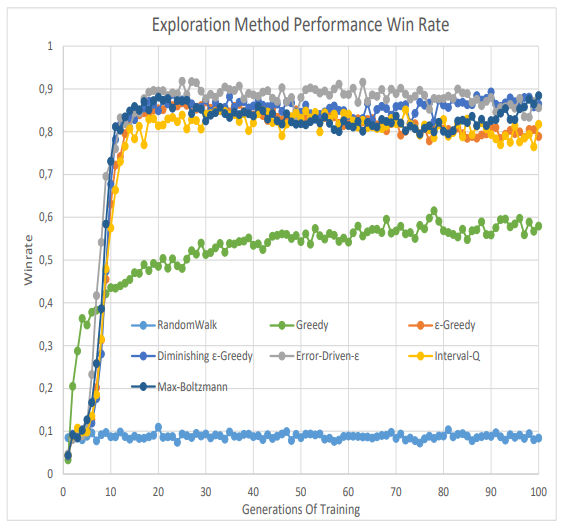
\includegraphics[width=0.6\linewidth]{figures/exploration.PNG}
	\caption{Comparison of different exploration methods}
	\label{fig:exploration}
\end{figure}

In the long run, Max Boltzmann performs best with 

\begin{equation}
	\Pi(s,a) = \frac{e^{Q(s,a)/T}}{\sum_i^{\abs{A}}e^{Q(s,a^i)/T}}
\end{equation}

and T being the temperature parameter. But as the result is based on 100 generations of training with each generation comprising 10.000 episodes, Diminishing $\epsilon$-Greedy as the second best exploration method was chosen as this exploration method converges faster in the early stages of training.

Two improvements where considered to optimize the exploration phase, but were discarded in the end. The first one is to replace the uniform sampling method by a multinomial sampling method in case an exploration step should be done, i.e. when a randomly generated number is smaller than $\epsilon$. This means the second best action would be chosen more often compared to other actions during the exploration phase. This could be beneficial especially in later phases of training in case the Q-values are close to each other. But esspecially in the beginning of the training phase this could lead towards an unintended bias towards specific actions as the exploration of others will be suppressed probabilistically.

The second improvement was to include an exploration function as \cite{Geron2018} proposes. A simple exploration function could be 

\begin{equation}
	f(q,n) = q + \frac{K}{1+n}
\end{equation}

with $q$ being the Q-value and $n$ being the count how often a specific action $a$ was chosen in state $s$. $K$ is a hyperparameter that determines the amount of curiosity during training. To implement this one would need to store $n$ for every state and action. But as the state is far too high dimensional in the Bomberman environment this would require a lot of training just as using the Max Boltzmann exploration method to be beneficial in the end. 

\begin{itemize}
	\item Experience buffer and sum tree
	\item Imitation learning
	\item Visualization with Tensorboard
	\item Rewards
	\item Hyperparameters
	\item Cloud training
\end{itemize}

